\part{Ziel \& Frage}
\label{part:goal}
\begin{frame}[fragile]{}
\usebeamerfont{frametitle}\textcolor{blue}{Ziel:} \usebeamerfont{text}HoloLens einsetzen, um Versuchsaufbau mit Informationen anzureichern.
\pause
\vskip 1em
\usebeamerfont{frametitle}\textcolor{blue}{Frage:} \usebeamerfont{text}Wie kann die HoloLens für diesen Versuch konkret eingesetzt werden?
\end{frame}

\part{Anforderungen}
\begin{frame}[fragile]{}
\begin{center}
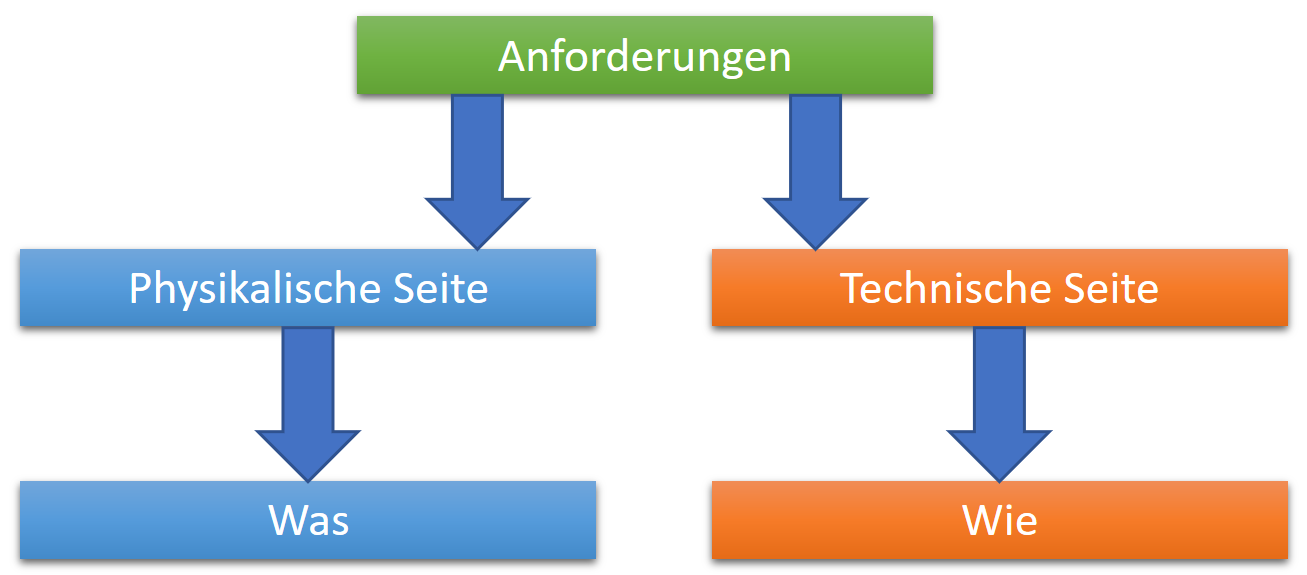
\includegraphics[width=0.9\textwidth]{images/Anforderungen.png}
\end{center}
\end{frame}

\part{Physikalische Seite}
\begin{frame}[fragile]{Anforderungen aus dem Anwendungsfall heraus}
\begin{itemize}
\item Magnetfeld von Erde und Spule
\begin{itemize}
\item Stärke
\item Richtung
\item Homogenität
\item Inhomogenität am Rand der Spule andeuten (Optional) 
\end{itemize}
\item Stromfluss durch die Spule
\begin{itemize}
\item Richtung
\item Kennzeichnung von Plus und Minus
\item Stärke (Optional) 
\end{itemize}
\end{itemize}
\end{frame}

\begin{frame}[fragile]{Anforderungen aus dem Anwendungsbereich}
\begin{itemize}
\setlength{\itemsep}{-0.25em}
\item Kompass
\begin{itemize}
\setlength{\itemsep}{-0.25em}
\item Nordrichtung
\item Grobe Auslenkung der Nadel
\end{itemize}
\item Weitere Informationen (Optional)
\begin{itemize}
\item Windungszahl der Spule
\item Durchmesser und Abstand der Spulen
\item Numerische Werte und Informationen (z.B. Fließt aktuell Strom, angelegte Stromstärke, angenommene Stärke des Erdmagnetfeldes, systematischer und zufälliger Fehler, etc.)
\end{itemize}
\end{itemize}
\end{frame}

\part{Technische Seite}
\label{part:tech}
\begin{frame}[fragile]{Möglichkeiten der HoloLens}
\begin{minipage}{0.5\textwidth}
	{\setstretch{1.0}
		\begin{itemize}[itemsep=1mm]
			\item Holografische Darstellungen
			\item Raumverständnis
			\item Raumklang
			\item Interaktion
			\item Softwareunterstützung
		\end{itemize}
	}
\end{minipage}
\begin{minipage}{0.48\textwidth}
	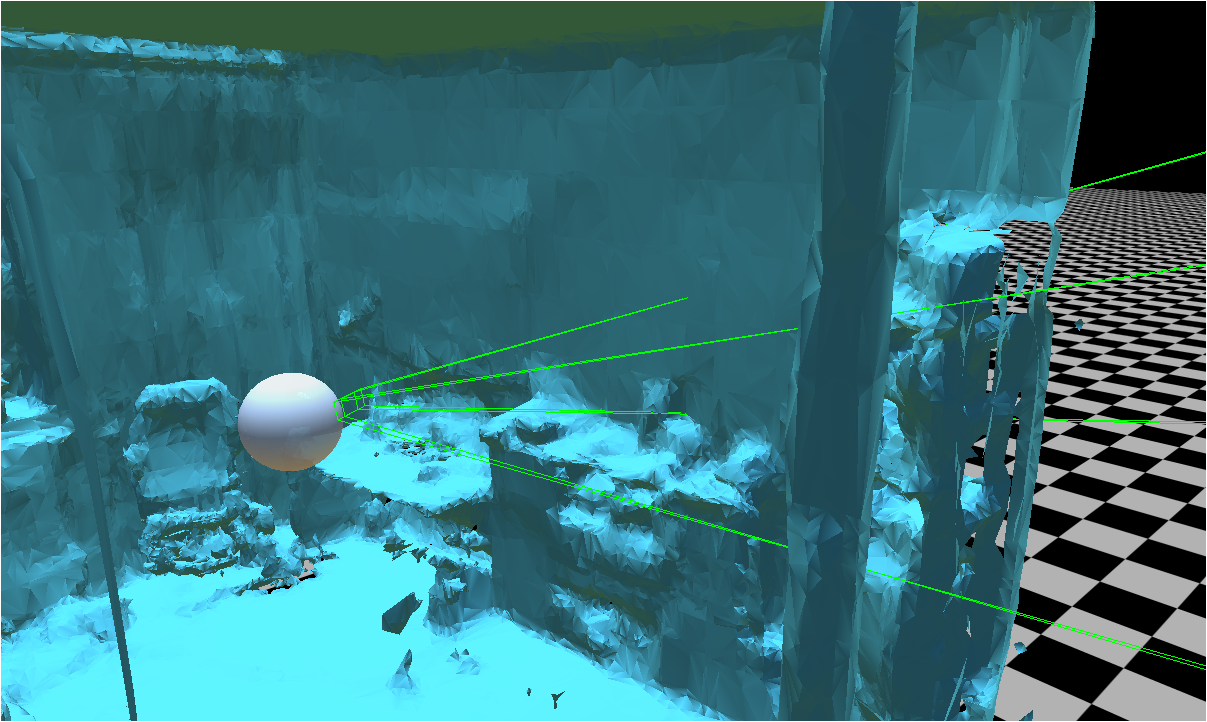
\includegraphics[width=0.9\textwidth]{images/Spatial_Understanding.png}
	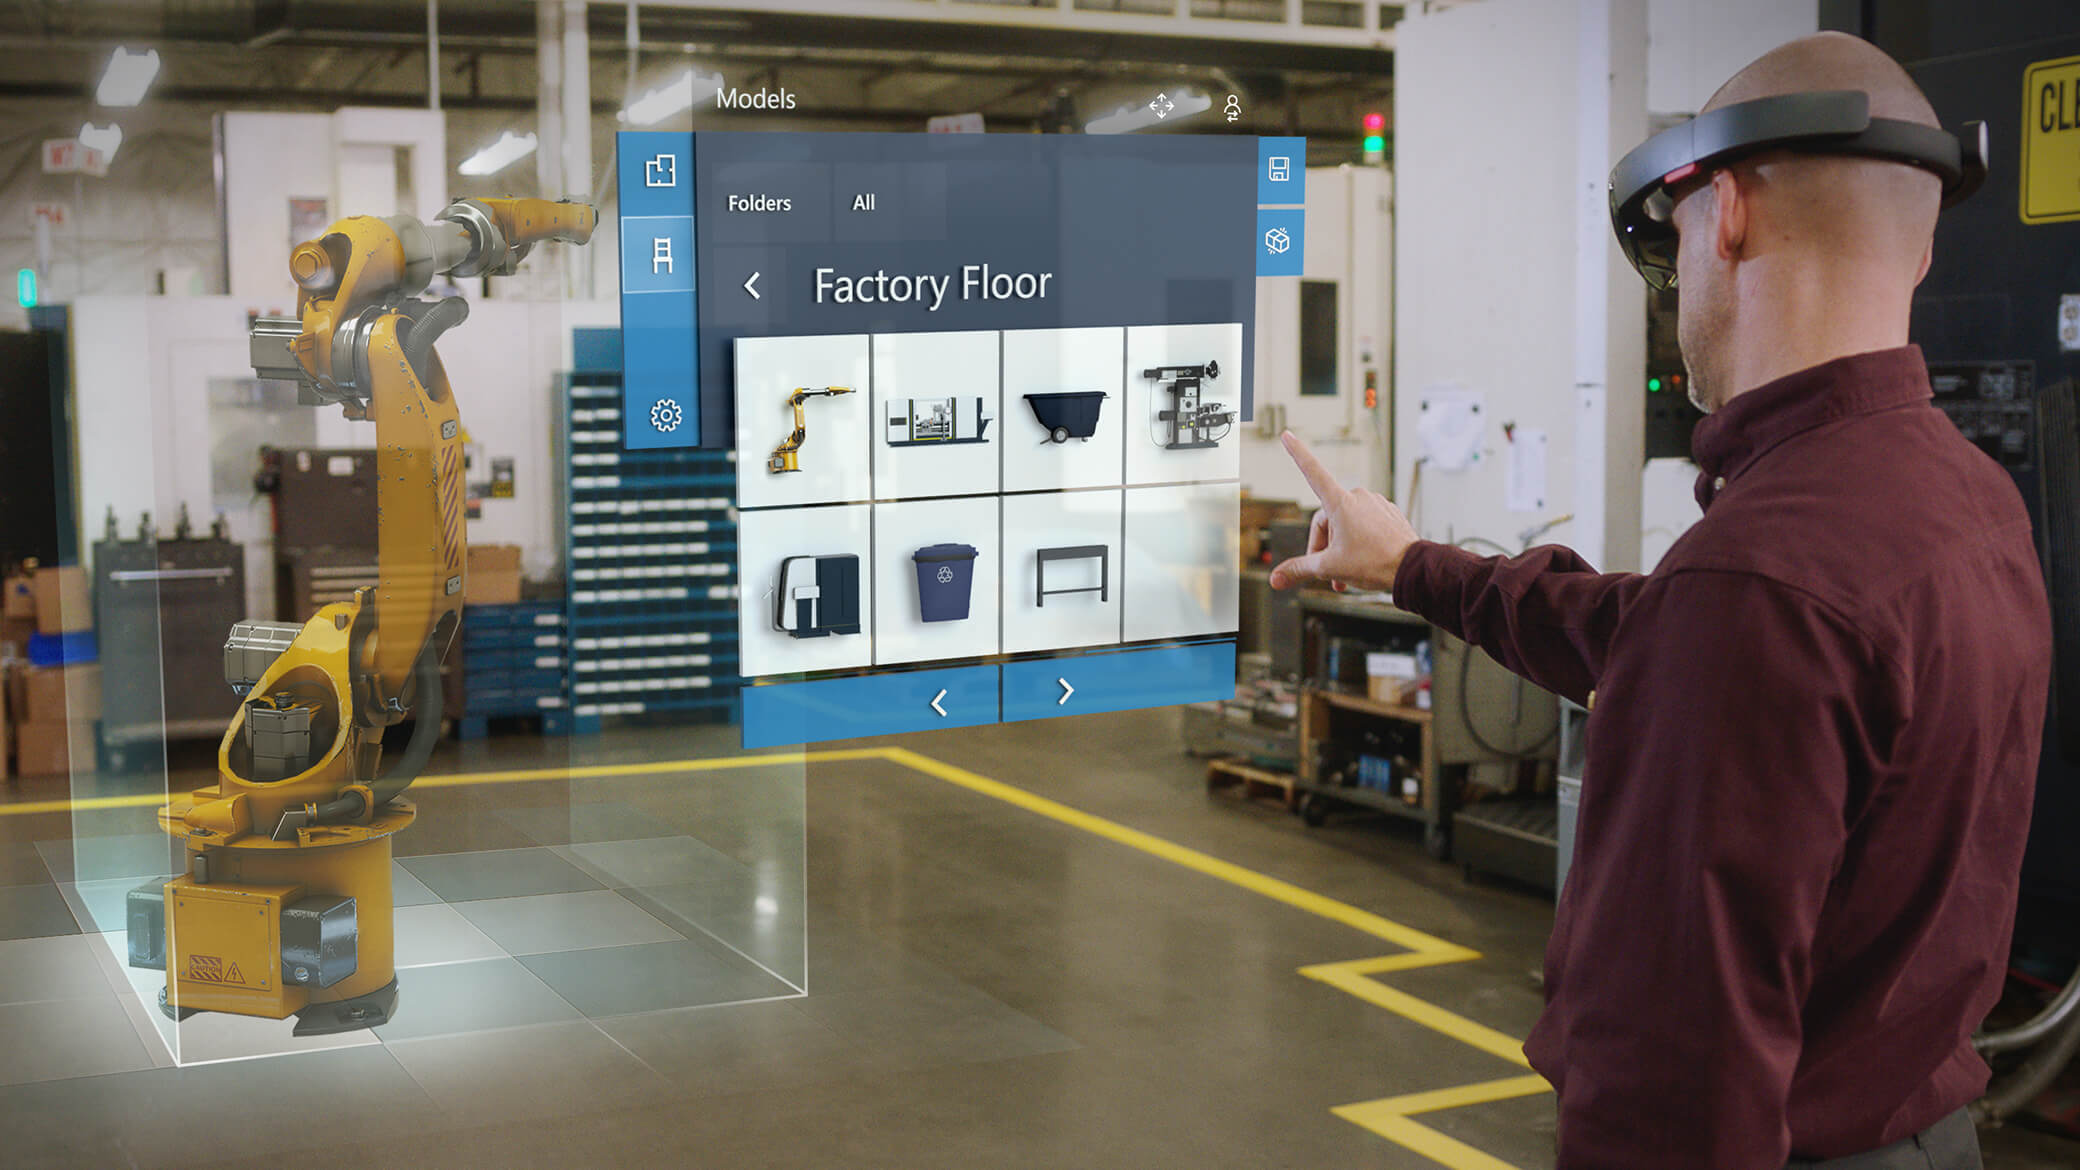
\includegraphics[width=0.9\textwidth]{images/HoloLens_Factory_Floor.jpg}
\end{minipage}
\end{frame}

\begin{frame}[fragile]{Anforderungen aus technischen Gegebenheiten}
\begin{itemize}
\item Größe, Geschwindigkeit, Farbe, Distanz zur Kamera von Objekten
\pause
\item Zusammenspiel der Darstellungen mit der Umgebung beachten
\pause
\item Stabilität der Hologramme gewährleisten
\pause
\item 60 FPS stabil halten, stark spiegelnde oder transparente Oberflächen vermeiden, mögliche Einflüsse auf die Sensoren beachten
\pause
\item Usability und UX Empfehlungen beachten
\end{itemize}
\end{frame}


\part{Problemstellung}
\label{part:golas}
\begin{frame}
\vspace{-1em}
\begin{center}
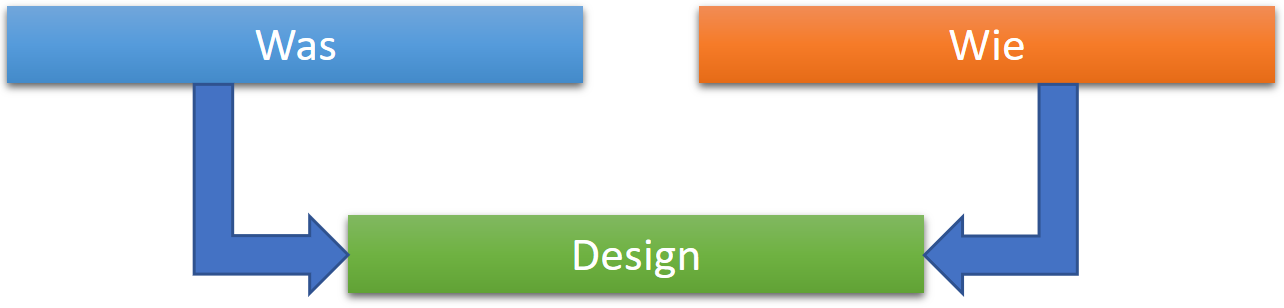
\includegraphics[width=0.8\textwidth]{images/Informiertes_Design.png}	
\end{center}
\usebeamerfont{frametitle}\textcolor{blue}{Fragen:}
\begin{itemize}
\item Was soll dargestellt werden?
\item Wie soll es dargestellt werden?
\item Wie soll damit interagiert werden?
\end{itemize}
\vspace{50px}
\end{frame}
